\section{eo\-One\-Max$<$ Fit\-T $>$ Class Template Reference}
\label{classeo_one_max}\index{eoOneMax@{eoOneMax}}
Always write a comment in this format before class definition if you want the class to be documented by Doxygen.  


{\tt \#include $<$eo\-One\-Max.h$>$}

Inheritance diagram for eo\-One\-Max$<$ Fit\-T $>$::\begin{figure}[H]
\begin{center}
\leavevmode
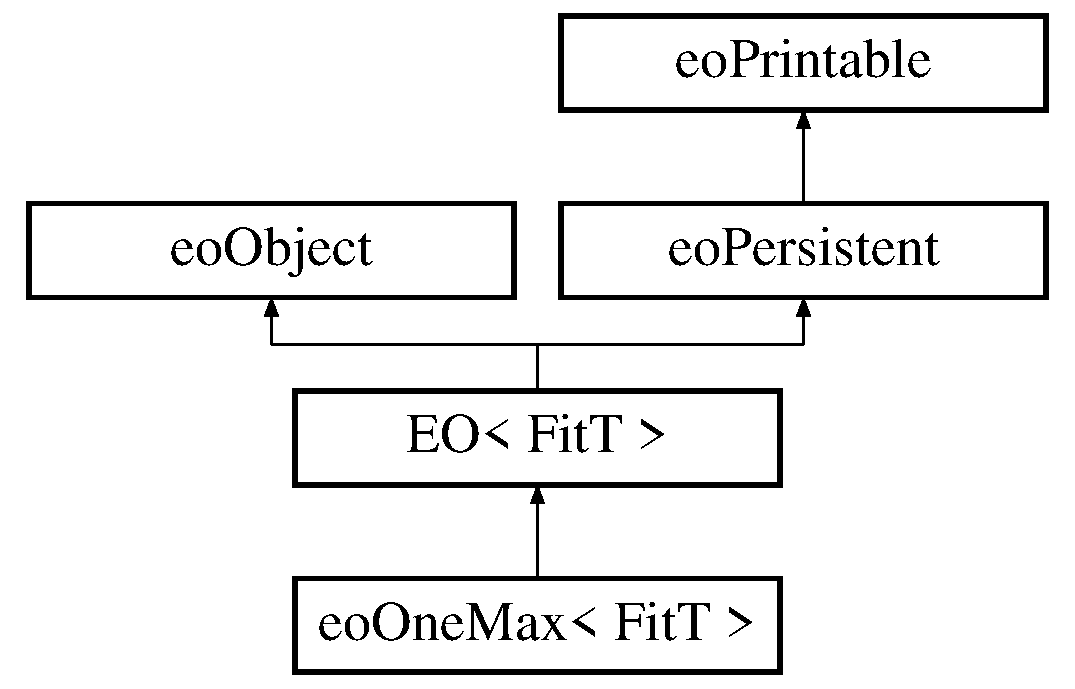
\includegraphics[height=4cm]{classeo_one_max}
\end{center}
\end{figure}
\subsection*{Public Member Functions}
\begin{CompactItemize}
\item 
{\bf eo\-One\-Max} ()
\begin{CompactList}\small\item\em Ctor: you MUST provide a default ctor. \item\end{CompactList}\item 
virtual string {\bf class\-Name} () const 
\begin{CompactList}\small\item\em Return the class id. \item\end{CompactList}\item 
void {\bf print\-On} (ostream \&\_\-os) const 
\begin{CompactList}\small\item\em printing... \item\end{CompactList}\item 
void {\bf read\-From} (istream \&\_\-is)
\begin{CompactList}\small\item\em reading... \item\end{CompactList}\item 
void {\bf set\-B} (vector$<$ bool $>$ \&\_\-b)\label{classeo_one_max_a5}

\item 
const vector$<$ bool $>$ \& {\bf B} ()\label{classeo_one_max_a6}

\end{CompactItemize}
\subsection*{Private Attributes}
\begin{CompactItemize}
\item 
std::vector$<$ bool $>$ {\bf b}\label{classeo_one_max_r0}

\end{CompactItemize}


\subsection{Detailed Description}
\subsubsection*{template$<$class Fit\-T$>$ class eo\-One\-Max$<$ Fit\-T $>$}

Always write a comment in this format before class definition if you want the class to be documented by Doxygen. 

Note that you MUST derive your structure from EO$<$fit\-T$>$ but you MAY use some other already prepared class in the hierarchy like {\bf eo\-Vector}{\rm (p.\,\pageref{classeo_vector})} for instance, if you handle a vector of something....

If you create a structure from scratch, the only thing you need to provide are a default constructor IO routines print\-On and read\-From

Note that operator$<$$<$ and operator$>$$>$ are defined at {\bf EO}{\rm (p.\,\pageref{class_e_o})} level using these routines 



Definition at line 31 of file eo\-One\-Max.h.

\subsection{Constructor \& Destructor Documentation}
\index{eoOneMax@{eo\-One\-Max}!eoOneMax@{eoOneMax}}
\index{eoOneMax@{eoOneMax}!eoOneMax@{eo\-One\-Max}}
\subsubsection{\setlength{\rightskip}{0pt plus 5cm}template$<$class Fit\-T$>$ {\bf eo\-One\-Max}$<$ {\bf Fit\-T} $>$::{\bf eo\-One\-Max} ()\hspace{0.3cm}{\tt  [inline]}}\label{classeo_one_max_a0}


Ctor: you MUST provide a default ctor. 

though such individuals will generally be processed by some {\bf eo\-Init}{\rm (p.\,\pageref{classeo_init})} object 

Definition at line 37 of file eo\-One\-Max.h.

\subsection{Member Function Documentation}
\index{eoOneMax@{eo\-One\-Max}!className@{className}}
\index{className@{className}!eoOneMax@{eo\-One\-Max}}
\subsubsection{\setlength{\rightskip}{0pt plus 5cm}template$<$class Fit\-T$>$ virtual string {\bf eo\-One\-Max}$<$ {\bf Fit\-T} $>$::class\-Name (void) const\hspace{0.3cm}{\tt  [inline, virtual]}}\label{classeo_one_max_a2}


Return the class id. 

\begin{Desc}
\item[Returns:]the class name as a std::string \end{Desc}


Reimplemented from {\bf EO$<$ Fit\-T $>$} {\rm (p.\,\pageref{class_e_o_z10_0})}.

Definition at line 49 of file eo\-One\-Max.h.\index{eoOneMax@{eo\-One\-Max}!printOn@{printOn}}
\index{printOn@{printOn}!eoOneMax@{eo\-One\-Max}}
\subsubsection{\setlength{\rightskip}{0pt plus 5cm}template$<$class Fit\-T$>$ void {\bf eo\-One\-Max}$<$ {\bf Fit\-T} $>$::print\-On (ostream \& {\em \_\-os}) const\hspace{0.3cm}{\tt  [inline]}}\label{classeo_one_max_a3}


printing... 

HINTS in {\bf EO}{\rm (p.\,\pageref{class_e_o})} we systematically write the sizes of things before the things so read\-From is easier to code (see below)

Definition at line 52 of file eo\-One\-Max.h.

References EO$<$ F $>$::print\-On().\index{eoOneMax@{eo\-One\-Max}!readFrom@{readFrom}}
\index{readFrom@{readFrom}!eoOneMax@{eo\-One\-Max}}
\subsubsection{\setlength{\rightskip}{0pt plus 5cm}template$<$class Fit\-T$>$ void {\bf eo\-One\-Max}$<$ {\bf Fit\-T} $>$::read\-From (istream \& {\em \_\-is})\hspace{0.3cm}{\tt  [inline]}}\label{classeo_one_max_a4}


reading... 

of course, your read\-From must be able to read what print\-On writes!!!

HINTS remember the eo\-One\-Max object will come from the default ctor this is why having the sizes written out is useful 

Definition at line 72 of file eo\-One\-Max.h.

References EO$<$ F $>$::read\-From().

The documentation for this class was generated from the following file:\begin{CompactItemize}
\item 
eo\-One\-Max.h\end{CompactItemize}
